\documentclass[10 pt,usenames,dvipsnames, oneside]{article}
\usepackage{../../modelo-fracoes}
\graphicspath{{../../../Figuras/licao01/}}


\begin{document}

\begin{center}
  \begin{minipage}[l]{3cm}

\includegraphics[width=2cm]{../../../Figuras/logo}       
\end{minipage}\hfill
\begin{minipage}[r]{.8\textwidth}
 {\Large \scshape Atividade: Qual é a unidade? (parte II)}  
\end{minipage}
\end{center}
\vspace{.2cm}

\ifdefined\prof
\begin{goals}
\begin{enumerate}

\item       Identificar uma mesma fração unitária (no caso, a terça parte) em representações diversas.

\end{enumerate}
\tcblower

\begin{itemize}
\item       Recomenda-se que esta atividade seja desenvolvida em grupos de 3 a 5 alunos.
\item       Durante a discussão, os alunos devem ser estimulados a explicar as suas escolhas. A discussão sobre os motivos da identificação, ou não, de cada uma das representações à terça parte da unidade correspondente será fundamental para atingir o objetivo da atividade.
\item       Os alunos devem reconhecer que, seja qual for a unidade considerada, em uma equipartição em 3 partes, cada uma das partes é um terço (ou a terça parte) da unidade.
\item       Aproveite as próprias palavras e os argumentos dos alunos para conduzi-los às conclusões esperadas.
\item       Fique atento aos alunos que selecionarem as figuras que simplesmente possuem alguma associação com o número 3, não correspondendo a terços. Por exemplo, um aluno que associe a       {\bf Figura f)} a terços pode ainda não ter compreendido a necessidade da equipartição para a identificação de um terço. Já o aluno que associa       {\bf Figura g)}       a terços pode estar simplesmente contando as partes em vermelho, sem que tenha reconhecido que a figura deveria estar dividida em 3 partes iguais e não em 5.
\end{itemize}


\end{goals}

\bigskip
\begin{center}
{\large \scshape Atividade}
\end{center}
\fi

Em cinco das figuras a seguir, a parte em vermelho é um terço da figura. Identifique essas figuras.

\begin{center}
\begin{longtable}{ccc}
a)
\parbox[t][3cm][c]{5cm}{
  \begin{tikzpicture}[scale=0.7]
    \draw[very thick, attention] (90:2 cm)  -- (210:2 cm);
    \draw[very thick, attention] (330:2 cm) -- (90:2 cm);
    \draw[very thick, common] (210:2 cm)  -- (330:2 cm);
  \end{tikzpicture}
}
& \quad \quad  &


b)
\parbox[t][3cm][c]{5cm}{
\begin{tikzpicture}[scale=0.7]
  \draw[very thick, common] (90:2 cm)  -- (210:2 cm);
  \draw[very thick, attention] (210:2 cm)  -- (330:2 cm);
  \draw[very thick, common] (330:2 cm) -- (90:2 cm);
\end{tikzpicture}
}
\\


c)
\parbox[t][3cm][c]{5cm}{
\begin{tikzpicture}[scale=4]
  \draw[very thick, common] (0,3) -- (3,0);
  \draw[very thick, attention] (3,0) -- (6,3);
  \draw[very thick, common] (6,3) -- (9,0);
\end{tikzpicture}
}
& &


d)
\parbox[t][3cm][c]{5cm}{
  \begin{tikzpicture}[scale=4]
    \draw[very thick, attention] (0,3) -- (3,0);
    \draw[very thick, attention] (3,0) -- (6,3);
    \draw[very thick, common] (6,3) -- (9,0);
  \end{tikzpicture}
}

\\
e)
\parbox[t][3cm][c]{5cm}{
\begin{tikzpicture}[scale=3]
    \draw[fill=common, fill opacity=.3] (0,0) rectangle (3,1);
    \draw[fill=attention] (3,0) rectangle (6,1);
    \draw[fill=common, fill opacity=.3] (6,0) rectangle (9,1);
\end{tikzpicture}
}
& &

f)
\parbox[t][3cm][c]{5cm}{
\begin{tikzpicture}[scale=3]
    \draw[fill=common, fill opacity=.3] (0,0) rectangle (2,1);
    \draw[fill=attention] (2,0) rectangle (6,1);
    \draw[fill=common, fill opacity=.3] (6,0) rectangle (9,1);
\end{tikzpicture}
}
\\
g)
\parbox[t][3cm][c]{5cm}{
\begin{tikzpicture}[scale=0.7]

\filldraw [fill=common, fill opacity=.3, draw=black] (0:2 cm) -- (90:2 cm) -- (180:2 cm) -- (0,0) -- ( (270:2 cm) --cycle;
\fill[attention] (180:2 cm) -- (270:2cm) -- (0,0) -- cycle;
\draw (180:2 cm) -- (0:2 cm);
\draw (90:2 cm) -- (270:2 cm);
\draw (180:2 cm) -- (270:2 cm);
\end{tikzpicture}
}
&&
h)
\parbox[t][3cm][c]{5cm}{
\begin{tikzpicture}[scale=0.7]
  \filldraw[fill=attention, draw=black] (-2 cm, 0) -- (0,0) -- (0, 2 cm) arc (90:180:2 cm) -- cycle;
  \filldraw[fill=common, draw=black, fill opacity=.3] (-2 cm, 0) -- (2 cm,0) arc (0:-180: 2cm);
  \fill (0,0) circle (2 pt);
\end{tikzpicture}
}
\\
i)
\parbox[t][3cm][c]{5cm}{
\begin{tikzpicture}[scale=6]
  \filldraw[fill=common, fill opacity=.3, draw=black] (0,0) -- (0.5,0.5) -- (4,0.5) -- (4,2) -- (4.5,2.5) -- (4.5,0)--cycle;
  \fill[attention] (0,0) -- (0.5,0.5) -- (0.5,2) -- (4,2) -- (4.5,2.5) -- (0,2.5)--cycle;
 \draw (0,0) rectangle (4.5,2.5);
  \draw (0.5,0.5) rectangle (4,2);
\end{tikzpicture}
}
& &


j)
\parbox[t][3cm][c]{5cm}{

%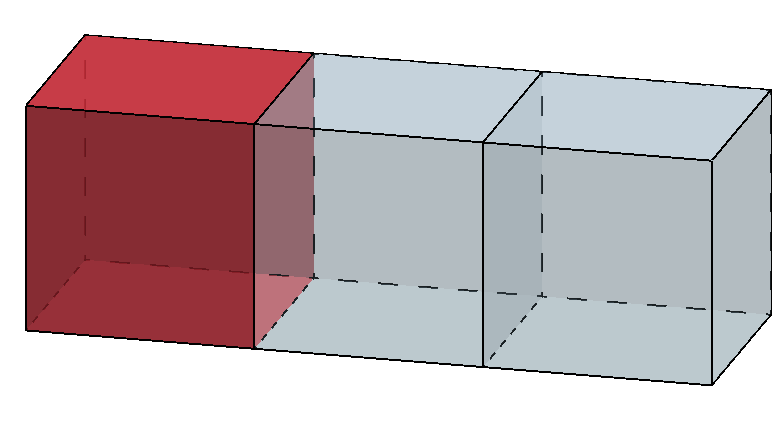
\includegraphics[scale=.6]{..figuras/licao01/paralelepipedo_tercos.png}
%}
  \begin{tikzpicture}%[scale=60]
  \tikzset{
  annotated cuboid/.pic={
    \tikzset{%
      every edge quotes/.append style={midway, auto},
      /cuboid/.cd,
      #1
    }
    \draw [every edge/.append style={pic actions, densely dashed, opacity=0}, pic actions]
    (0,0,0) coordinate (o) -- ++(-\cubescale*\cubex,0,0) coordinate (a) -- ++(0,-\cubescale*\cubey,0) coordinate (b) edge coordinate [pos=1] (g) ++(0,0,-\cubescale*\cubez)  -- ++(\cubescale*\cubex,0,0) coordinate (c) -- cycle
    (o) -- ++(0,0,-\cubescale*\cubez) coordinate (d) -- ++(0,-\cubescale*\cubey,0) coordinate (e) edge (g) -- (c) -- cycle
    (o) -- (a) -- ++(0,0,-\cubescale*\cubez) coordinate (f) edge (g) -- (d) -- cycle;
 },
  /cuboid/.search also={/tikz},
  /cuboid/.cd,
  width/.store in=\cubex,
  height/.store in=\cubey,
  depth/.store in=\cubez,
  units/.store in=\cubeunits,
  scale/.store in=\cubescale,
  width=100,
  height=100,
  depth=100,
  units=cm,
  scale=.1,
}

    \pic [fill=attention] at (50,0) {annotated cuboid={width=100, height=100, depth=14}};
    \pic [fill=common, fill opacity=.3] at (70,0) {annotated cuboid={width=200, height=100, depth=14}};
    \draw [dashed, lightgray] (50,-10,-1.4) -- (70,-10,-1.4);
    \draw [dashed, lightgray] (60,-10,0) -- (60,-10,-1.4) -- (60,0,-1.4);
    \draw [dashed] (60,0,-1.4) -- (60,0,0) -- (60,-10,0);
    \end{tikzpicture}
}


\end{longtable}
\end{center}


\ifdefined\prof

\begin{solucao}

A parte em vermelho representa um terço da figura nos itens b), c), e), h) e j).


\end{solucao}
\fi

\end{document}